\documentclass[fullscreen, unicode, bookmarks = false]{beamer}
\usetheme{default}

\usepackage[utf8]{inputenc}
\usepackage[english,russian]{babel}
\usepackage{amsmath,amsfonts,amssymb}
\usepackage{tikz}
\usepackage{tabularx}
\usepackage{hyperref}

\title{Проект TeachMe}
\author{
	Федор Амосов, СПбГУ \\
    Марк Ежков, СПбГУ	\\
    Екатерина Соса, СПбГУ	\\
    Дмитрий Харьковский, СПбГУ	\\~\\
    Руководители:	\\ 
    Александр Константинов, JetBrains \\
    Дмитрий Качмар, Яндекс	\\ 
}
\date{26 сентября 2013 г.}

\begin{document}

    \tikzstyle{thinline}=[gray,very thin]
    \tikzstyle{emphline}=[red,thick]

    \begin{frame}
        \titlepage
    \end{frame}

    \begin{frame}{Что за проект?}
        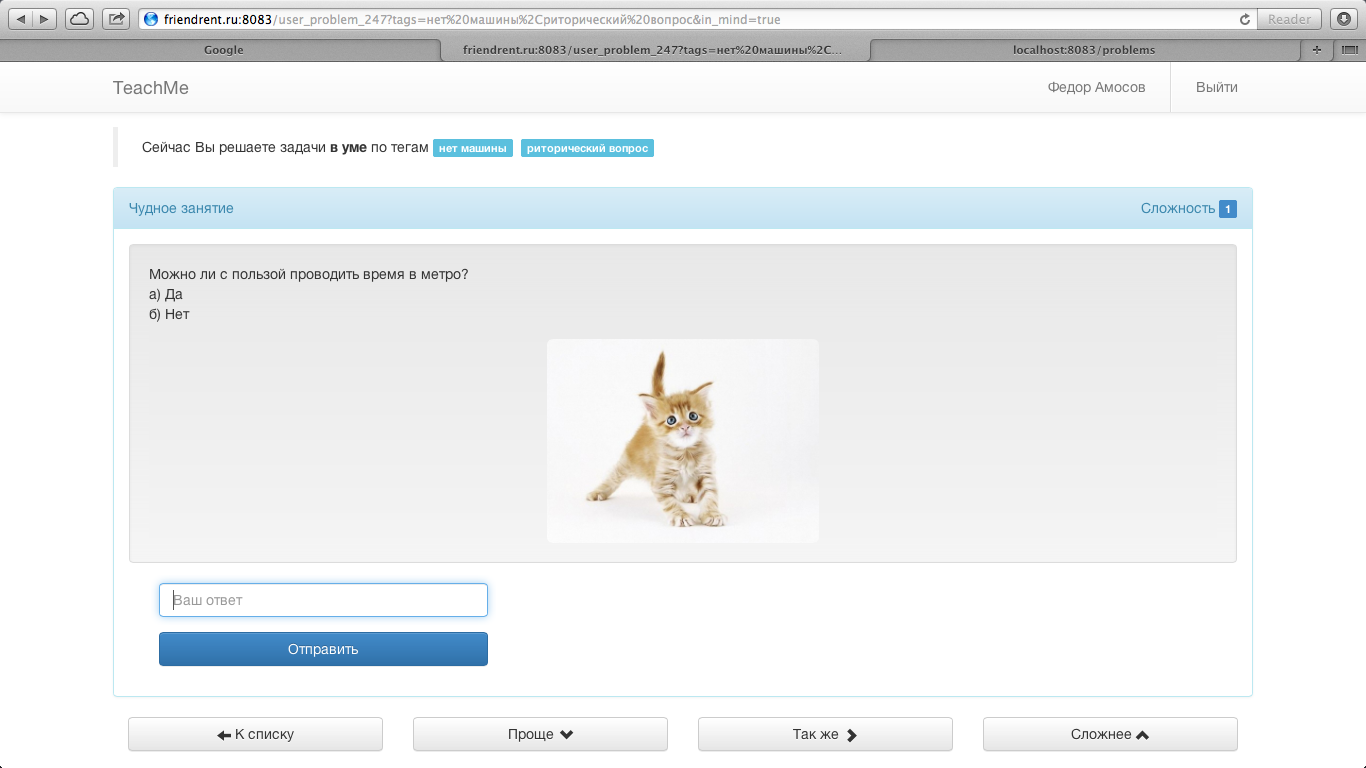
\includegraphics[scale=0.23]{metro1.png}
    \end{frame}
    \begin{frame}{Что за проект?}
        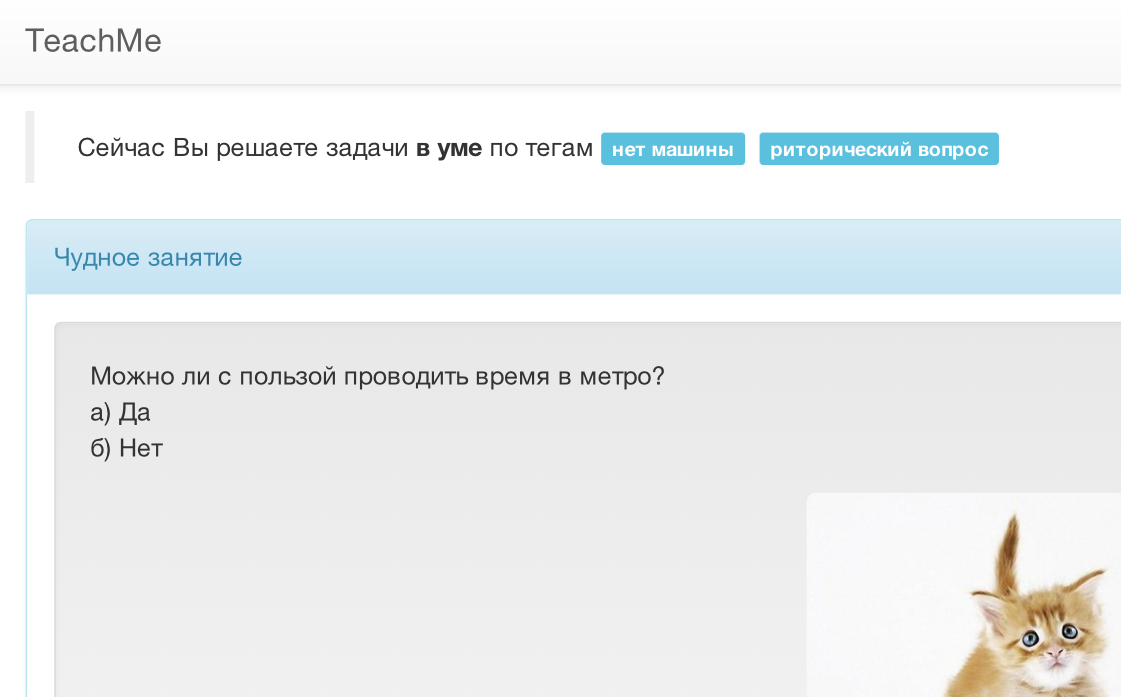
\includegraphics[scale=0.27]{metro2.png}
    \end{frame}
    \begin{frame}{Что за проект?}
        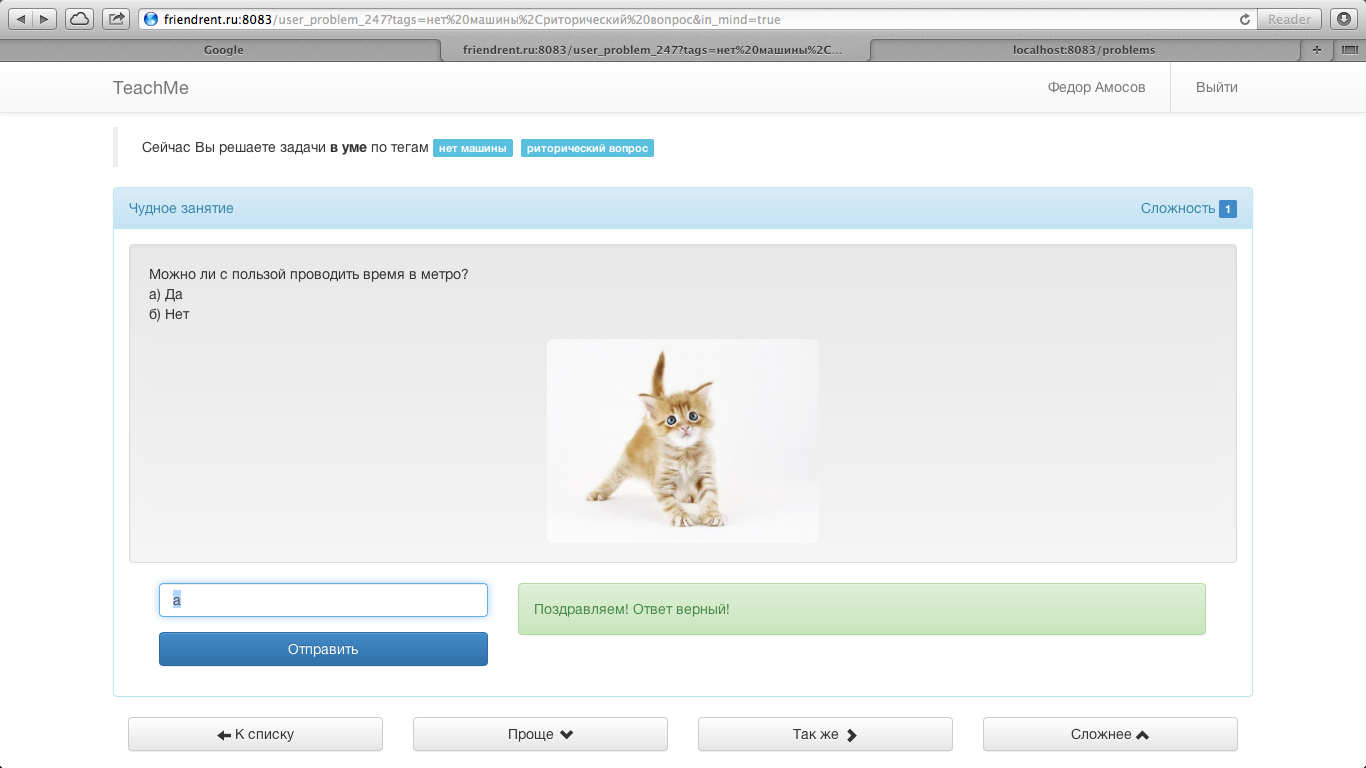
\includegraphics[scale=0.23]{metro3.png}
    \end{frame}
    %\begin{frame}{Что за проект?}
    %    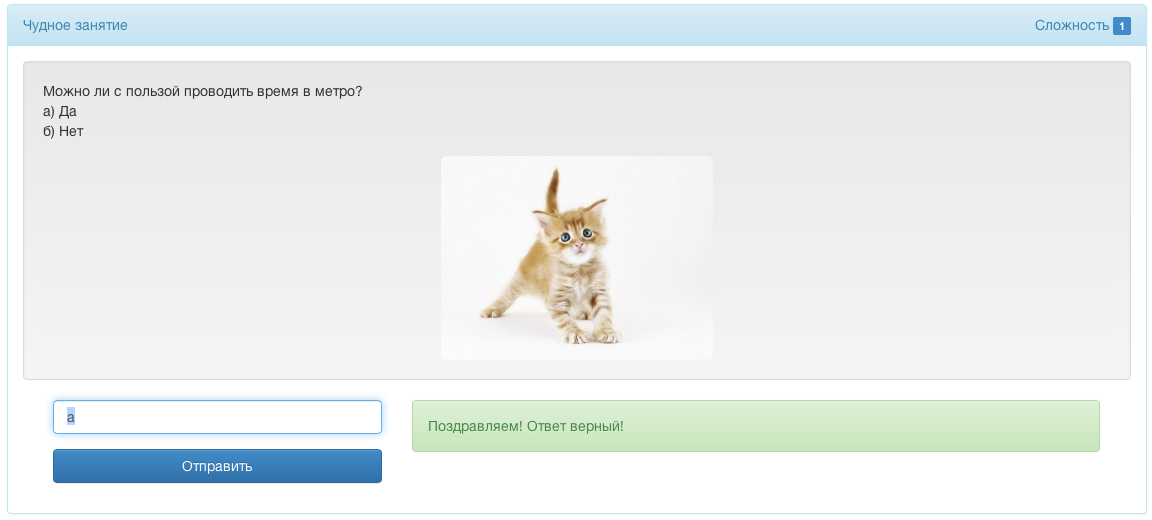
\includegraphics[scale=0.27]{metro4.png}
    %\end{frame}
    
    \begin{frame}{Фишка}
        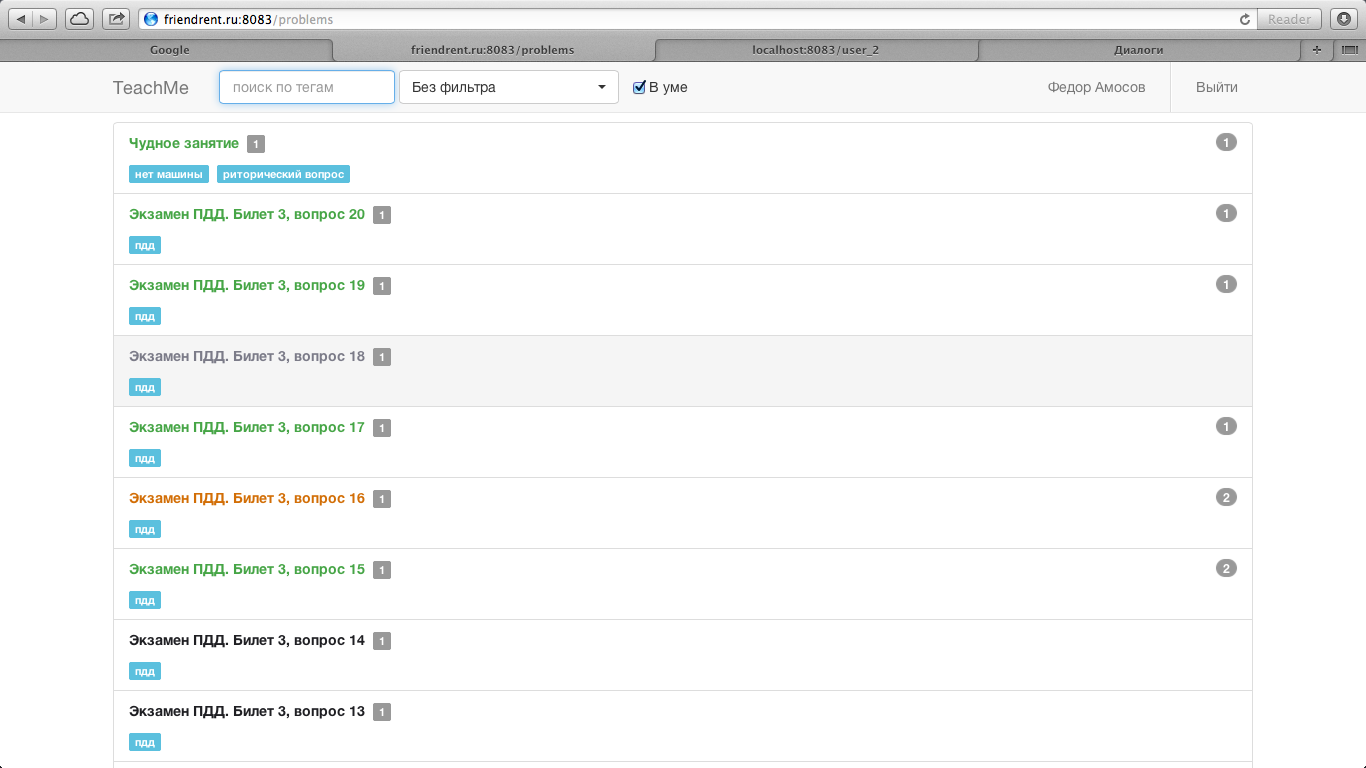
\includegraphics[scale=0.23]{fish1.png}
    \end{frame}
    \begin{frame}{Фишка}
        ~~~~~~~~~~~~~~~~~~~~~~~~
\includegraphics[scale=0.5]{fish2.png}
    \end{frame}
    \begin{frame}{Фишка}
        ~~~~~~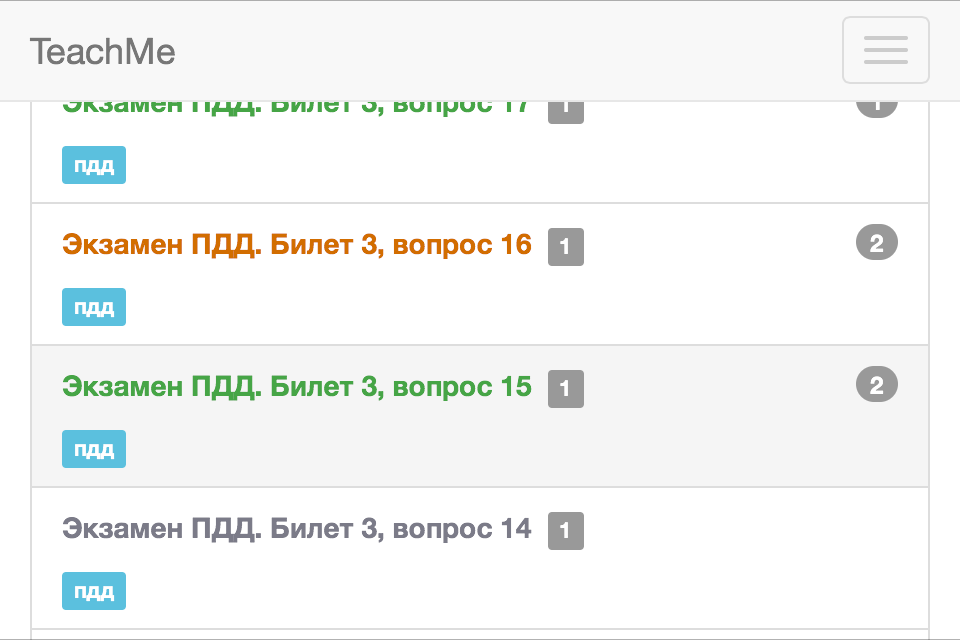
\includegraphics[scale=0.27]{fish25.png}
    \end{frame}
    \begin{frame}{Фишка}
        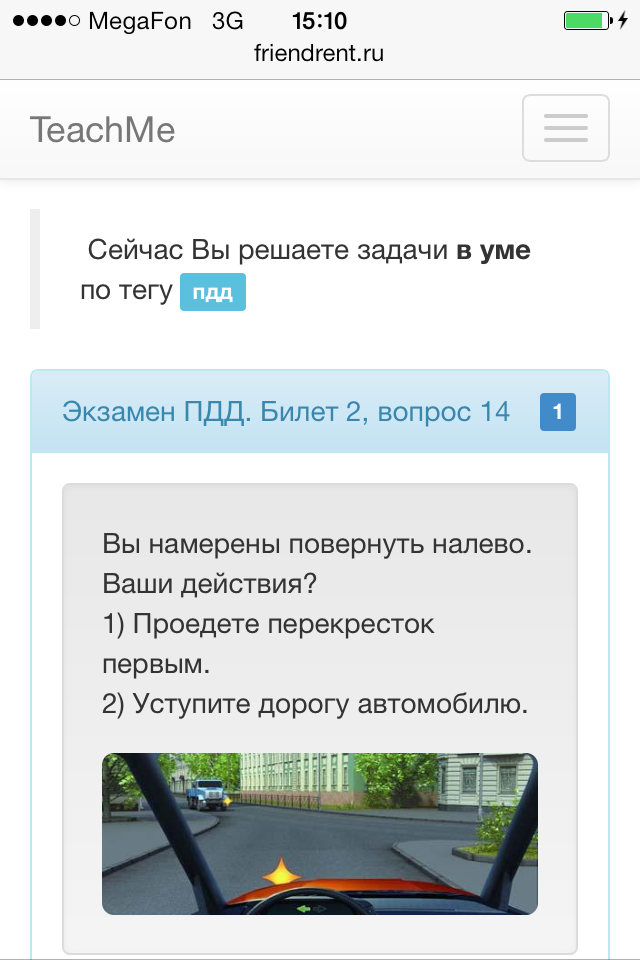
\includegraphics[scale=0.22]{fish31.png}~~~~~
        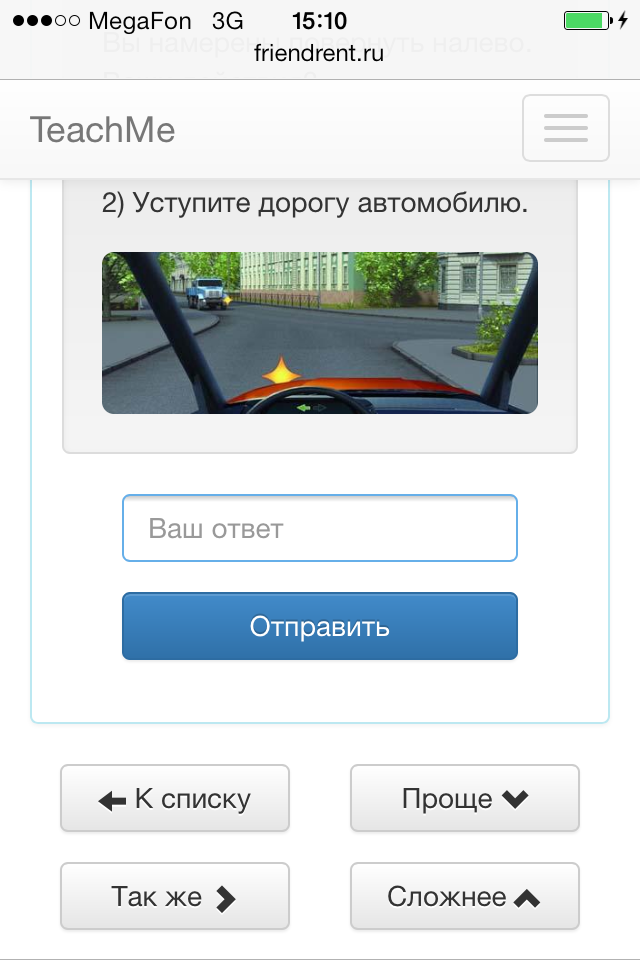
\includegraphics[scale=0.22]{fish32.png}
    \end{frame}
    %\begin{frame}{Фишка}
    %    
\includegraphics[scale=0.23]{fish41.png}\\
    %    
\includegraphics[scale=0.23]{fish42.png}
    %\end{frame}
        
    \begin{frame}{Серьезные задачи}
        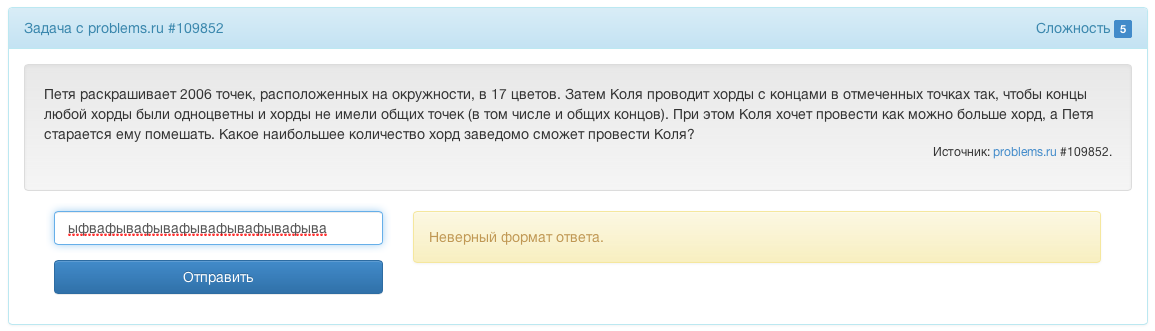
\includegraphics[scale=0.27]{serious.png}
    \end{frame}
    
    \begin{frame}{На чем написано}
        \begin{description}
            \item [Сервер]
                \begin{itemize}
                    \item Java + {\bf Spring Framework} + {\bf Jetty}
                    \item Maven
                    \item {\bf Spring JDBC} + {\bf MySql}
                    \item {\bf Spring MVC} + {\bf JSP}
                \end{itemize}
            ~\\
            \item [Клиент]
                \begin{itemize}
                    \item {\bf HTML} + {\bf CSS} + {\bf Bootstrap}
                    \item {\bf JavaScript} + {\bf jQuery} + {\bf Ajax} 
                \end{itemize}
            ~\\
            \item [Система контроля версий]
                \begin{itemize}
                    \item Git
                \end{itemize}
        \end{description}
    \end{frame}
    
    \begin{frame}{Авторизация}
		~~~~~~~~~~~~~~~~~
\includegraphics[scale=0.22]{login.png}
	\end{frame}
    
    \begin{frame}{Плагин для jQuery}
        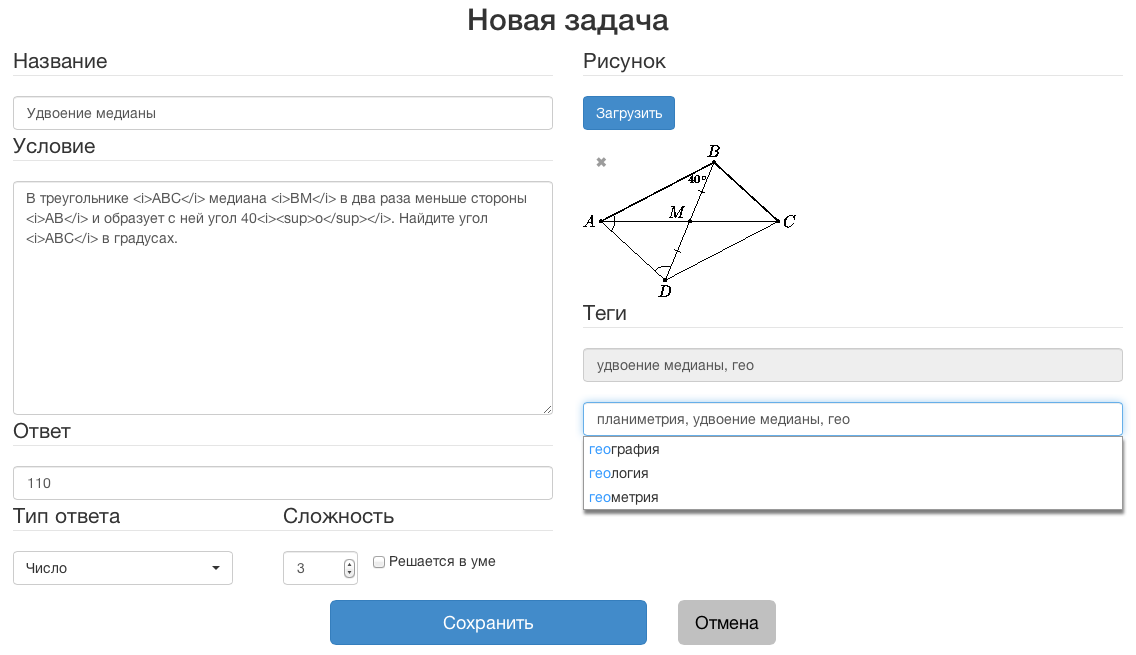
\includegraphics[scale=0.27]{plugin1.png}
    \end{frame}
    \begin{frame}{Плагин для jQuery}
        
\includegraphics[scale=0.23]{plugin21.png}\\
        ~\\
        
\includegraphics[scale=0.23]{plugin22.png}
    \end{frame}
     
    %\begin{frame}{Мобильная верстка}
    %    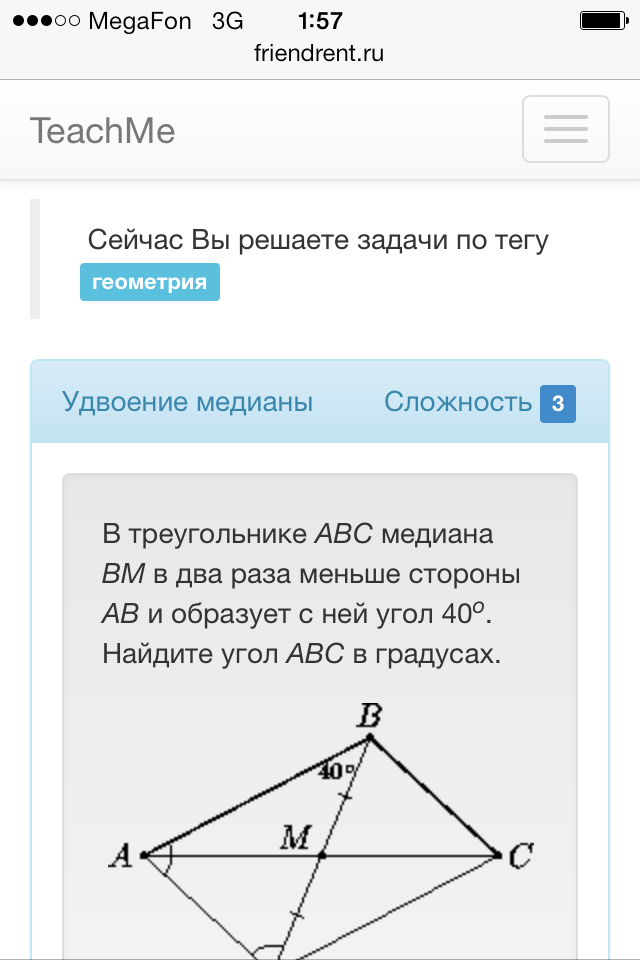
\includegraphics[scale=0.22]{mobile11.png}~~~~~
    %    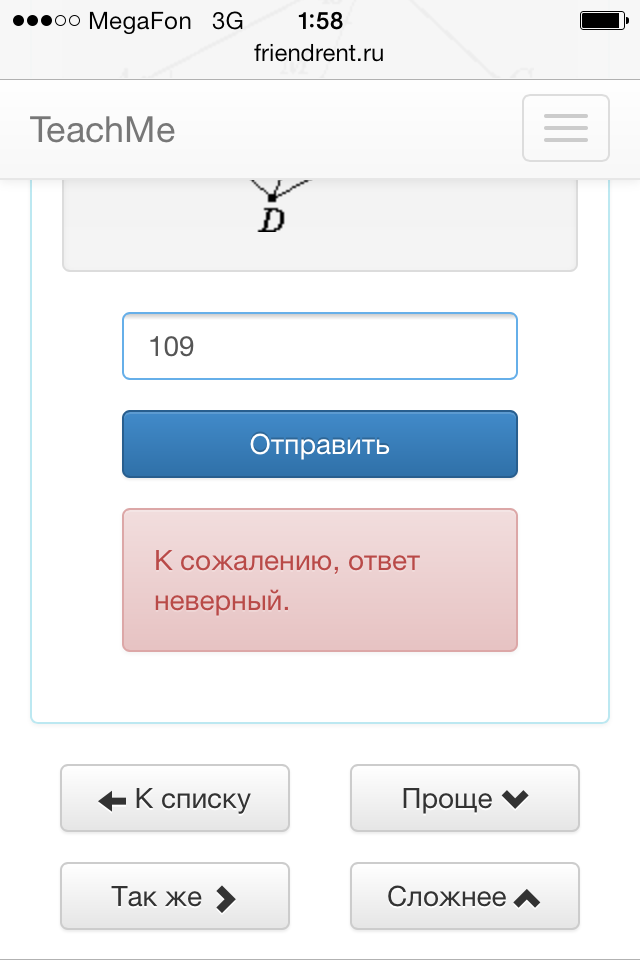
\includegraphics[scale=0.22]{mobile12.png}
    %\end{frame}
    
    \begin{frame}{Контент}
        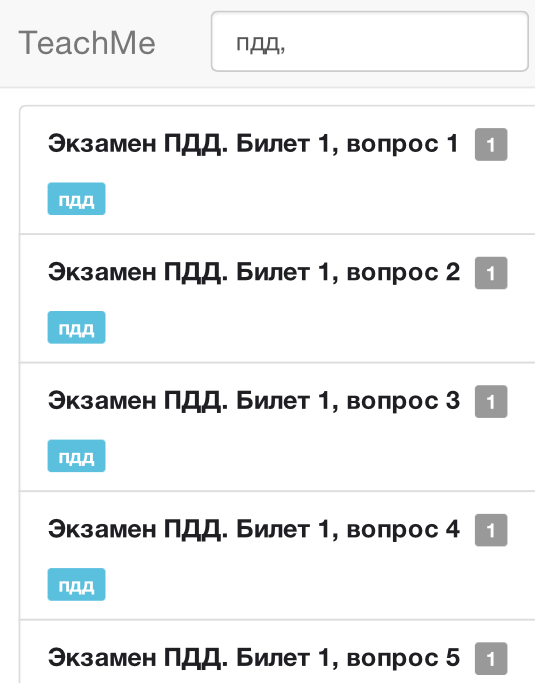
\includegraphics[scale=0.22]{pdd.png}~~~~~~
	    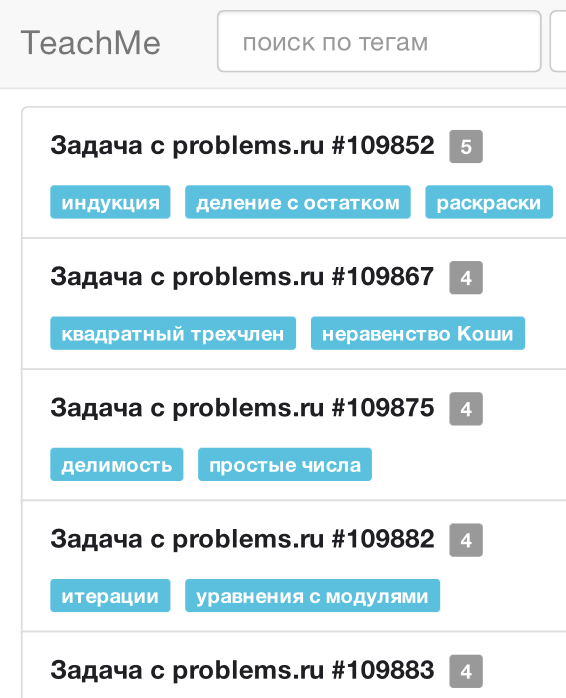
\includegraphics[scale=0.21]{problems.png}
		~\\~\\	    
	    
	    $800$ вопросов ПДД + $317$ с problems.ru = $1117$ задач        
    \end{frame}
     
    
	

    \begin{frame} {Q\&A}
		\begin{center}
        	Спасибо за внимание!\\
        	\textcolor{blue}{http://friendrent.ru:8083/}
		\end{center}
    \end{frame}

\end{document}
